\section{Projektplan}
\subsection{Teoretisk bakgrund}
När ett tåg ska svänga finns det flera aspekter som måste tas hänsyn till, där kurvradien och hastigheten är två av dem. Om denna radie är för liten eller om tågets hastighet är för hög kommer tåget vältas. Detta eftersom centrifugalkraften flyttar tyngdpunkten så den överskrider rotationsaxeln.
\subsection{Syfte}
Beskriv här syftet, alltså varför ni vill göra just i den här undersökningen, vad ni vill uppnå med resultaten eller hur resultaten kan bidra till förståelsen av det generella problem ni skrivit om i den teoretiska bakgrunden. Här skriver ni vad ni vill uppnå med ert gymnasiearbete. Ni kan till exempel börja med: Syftet med vårt gymnasiearbete är att beskriva/förklara/utvärdera/förstå … Beskriv också här kort hur ni planerar att uppnå syftet med arbetet. Ni kan till exempel skriva: I det här arbetet kommer vi att undersöka …
Längd: Ett par meningar

\subsection{Frågeställning}
\textbf{Fråga:} ''Vad är den maximala hastigheten ett modelltåg i skala 1:40 kan uppnå vid en given kurvradie utan att spåra ur?''

\begin{figure}[h!]
    \centering
    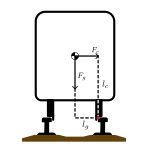
\includegraphics[width=0.33\textwidth]{fig/tåg_krafter.png}
    \caption{Kraftsituationen på en järnvägsvagn vid en vänstersväng där $F_g$ är tyngdkraften, $F_c$ är centrifugalkraften och $l_g$ respektive $l_c$ är deras momentarmar till rotationsaxeln A.}
    \label{fig:tåg_krafter_sväng}
\end{figure}

\subsection{Empirisk metod}
Materialen som kommer användas under undersökningen kommer vara: ett 3D printad tåg som väger ca 1,4 kg, en kamera som filmar i minst 240 FPS, ett stativ för att hålla kameran, rutat papper (med sidlängd 1 cm), 3D printade rälssegment.

Undersökningen kommer ske genom att det först väljs en viss radie. Därefter kommer tåget placeras på toppen av en backe med bestämd höjd. Målet med detta är att ge tåget en bestämd hastighet baserad på potentiell energi överförd till kinetisk energi. Sedan släpps tåget och resultaten från kameran och om den spårade ur eller ej skrivs ned. Om tåget inte har spårat ur kommer tåget placeras på en högre höjd och denna process repeteras tills tåget spårar ur. När tåget spårat ur välj en ny radie på kurvan och hela processen börjar om från början. När alla radier har testats kommer data skrivas in i en graf där hastigheten och radien är grafens axlar.



\subsection{Tidsplan}
vecka 40:
göra klart Projektplans utkastet och beställa kullager samt axlar till tågmodellen

Vecka 41: senaste dagen att lämna in projektplanen (måndag kl 1200) samt renskrivning av projektplan och mer inläsning av fysikaliska och matematiska modeller. utöver detta kada klart tågmodellen

vecka 42: samma som tidigare

vecka 43: inlämning av slutlig Projektplan

Vecka 44: höstlov

vecka 45: slutliga förberedelser för labben och ihopsättning/ kontrollering av modellens kvalite

vecka 46: om modellen visar sig vara av sämre kvalite; bygg om modellen, annars påbörja labben

vecka 47: avslutning/replikat av labben och eller formatering av data.

vecka 48: analys av data

vecka 49: formulera resultat

vecka 50: workshop statistik med excel

vecka 51-1: lov

vecka 2: genomgång felanalys

vecka 3: fortsätt bearbeta resultat och börja med att skriva ned dem

vecka 4: skriva resultat och diskussion

vecka 5: genomgång av naturvetenskaplig rapport och börja skriva resultat och diskussion

vecka 6: fortsätt skriva och börja med abstrakt när vi blir klara med tidigare delar

vecka 7: fortsätt skriva

vecka 8: fortsätt skriva

vecka 9: lov/kris skrivning

vecka 10: genomgång av hur oppositionen går till samt skrivning

vecka 11: inlämning av raport inför oppositionen

vecka 12: förberedelse av oppositionen

vecka 13: oppositioner

vecka 14: oppositioner

vecka 15: lov

vecka 16: revidering av rapport

vecka 17: gymnasiearbetes dag med åk 2

vecka 18: slutinlämning av rapport och allt annat (slut)